\documentclass[journal=esthag,manuscript=article]{achemso}

% additional packages
\usepackage[utf8]{inputenc}
\usepackage{amsmath}
\usepackage{booktabs}
\usepackage{subcaption}
\usepackage{tabularx}
\usepackage{array,multirow,graphicx}
\usepackage{comment}
\graphicspath{
  {./../figures/},
  {./../figures/2d_kde/},
  {./../figures/simulation_predictions/},
  {./../figures/pair_grids/},
  {./../figures/temporal_variability/},
}
\usepackage{lineno}
\linenumbers
% macros

% authors
\author{Jonathan G. V. Ström}
\affiliation[Brown University]{Brown University, School of Engineering, Providence, RI, USA}
\author{Yijun Yao}
\affiliation[Brown University]{Brown University, School of Engineering, Providence, RI, USA}
\author{Eric M. Suuberg}
\email{eric_suuberg@brown.edu}
\affiliation[Brown University]{Brown University, School of Engineering, Providence, RI, USA}

% title
\title{Temporal Variations In Vapor Intrusion Induced Indoor Air Contaminant Concentrations }

% keywords
\abbreviations{VI}
\keywords{Vapor intrusion, Preferential pathways, Temporal variability, Factor analysis, Modeling}

\begin{document}

\begin{abstract}

\end{abstract}

\section{Introduction}

Long term vapor intrusion (VI) studies in both residential and larger commercial structures have raised concerns regarding significant observed transient behavior in indoor air contaminant concentrations\cite{u.s._environmental_protection_agency_oswer_2015,folkes_observed_2009,holton_temporal_2013,johnston_spatiotemporal_2014,hosangadi_high-frequency_2017,mchugh_recent_2017,u.s._environmental_protection_agency_assessment_2015}.
Such variations make it difficult for those charged with protecting human health to formulate a response should evaluation of the risk of exposure be based upon observed peak concentrations, or long-term averages, or something else?
There is even uncertainty within the VI community regarding how to best develop sampling strategies to address this problem\cite{u.s._environmental_protection_agency_oswer_2015,holton_temporal_2013,johnson_integrated_2016}.
What represents a reasonable sampling strategy for a particular site a single 8 hr sample?
Repeated 8 hr samples?
Month-long samples?
Continuous monitoring?

VI involves the migration of volatilizing contaminants from soil, groundwater or other subsurface sources into overlying structures.
The basic nature of VI has been understood for some time and it has been the subject of much study, but some aspects remain poorly understood, such as the causes of the sometimes observed large temporal transients in indoor air concentrations.
Results from a house operated by Arizona State University (ASU) near Hill AFB in Utah, an EPA experimental house in Indianapolis, IN and a large warehouse at the Naval Air Station (NAS) North Island, CA have all shown significant transient variations in indoor air contaminant concentrations.
All were outfitted with sampling and monitoring equipment that allowed tracking temporal variation in indoor air contaminant concentrations on time scales of hours.
All have shown that these concentrations vary significantly with time - orders of magnitude on the timescale of a day or days\cite{holton_evaluation_2015,guo_vapor_2015,hosangadi_high-frequency_2017}.

In one instance the source of the variation was clearly established during the study of the site.
At the ASU house a drain pipe (or “land drain”) connected to a sewer system was discovered beneath the house.
Careful isolation of this source led to a clear conclusion that this “preferential pathway” for contaminant vapor migration significantly contributed to observed indoor air contaminant levels and their fluctuations\cite{guo_vapor_2015,guo_identification_2015}.
While in this case the issue of a contribution from a preferential pathway was clearly resolved, what it left open was a question of whether existence of such a preferential pathway would always be expected to lead to large fluctuations in indoor air contaminant concentrations.

Similarly, a sewer pipe has recently been suggested to be a source of the contaminants found in the EPA Indianapolis house.
That site was also characterized by large indoor air contaminant concentration fluctuations\cite{mchugh_evidence_2017,u.s._environmental_protection_agency_assessment_2015}.
Sewer lines have been previously implicated as VI sources at several sites\cite{pennell_sewer_2013,mchugh_evidence_2017,roghani_occurrence_2018,riis_vapor_2010}.
A Danish study has estimated that roughly 20\% of all VI sites in central Denmark involve significant sewer VI pathways\cite{nielsen_remediation_2017}.
Thus while consideration of sewer or other preferential pathways is now part of normal good practice in VI site investigation\cite{u.s._environmental_protection_agency_oswer_2015}, it is still not known whether the existence of such pathways automatically means that large temporal fluctuations are necessarily to be expected.

In some of the above cited cases\cite{pennell_sewer_2013,riis_vapor_2010}, a sewer provided a pathway for direct entry of contaminant into the living space.
While potentially important in many instances, this scenario is not further considered here where the focus is on pathways that deliver contaminant via the soil beneath a structure.
It is, however, now known that even absent a preferential pathway, there may be significant transient variation in indoor air contaminant concentrations at VI sites\cite{folkes_observed_2009,brenner_results_2010,johnston_spatiotemporal_2014}.
One example is the site at NAS North Island at which no preferential pathways have been identified.
Instead, a building at this site is characterized by significant temporal variations in indoor-outdoor pressure differential\cite{hosangadi_high-frequency_2017}.
It is believed that this is the origin of the observed indoor air contaminant concentration fluctuations at that site.

This paper investigates the sources of the temporal variation in indoor air contaminant concentrations in both the presence and absence of preferential pathways.
In this work, the latter scenarios are referred to as “normal” VI scenarios, in which there is typically a groundwater source of the contaminant.
Specifically, we pose the question of just how much variation in indoor air contaminant concentration may be expected at such normal VI sites vs. those characterized by preferential pathways within the soil beneath the site.
The conditions required for preferential pathways to become significant contributors to temporal variations in indoor air contaminant concentrations are also explored, and the consequences for sampling strategies are discussed.

\section{Methods}


\subsection{Statistical Analysis Of Field Data}

To frame the question of just how much variability in indoor air contaminant concentrations is actually seen, field datasets have been analyzed.
For this purpose, datasets from the ASU house in Utah, the EPA Indianapolis site and North Island NAS were chosen for analysis.
Readers are referred to the original published works for details regarding data acquisition\cite{holton_evaluation_2015,guo_vapor_2015,holton_temporal_2013,hosangadi_high-frequency_2017,u.s._environmental_protection_agency_assessment_2015}.

The ASU house data were obtained over a period of several years.
During part of this time, controlled pressure method (CPM) tests were being conducted, in which the house was underpressurized to an extent greater than that characterizing “normal” house operation thus increasing VI potential\cite{mchugh_evaluation_2012,mchugh_recent_2017,holton_evaluation_2015}.
The period of CPM testing is thus excluded from the analysis.
Likewise, the existence of a preferential pathway at the ASU house needs to be considered in examining that dataset; during some of the testing at that site, this pathway was cut off, resulting in “normal” VI conditions in which the main source of contaminant was diffusion of contaminant vapor from an underlying groundwater source.

The NAS North Island dataset has not (as far as is known) been influenced by a preferential pathway, but the structure there was subject to “large” internal pressure fluctuations.
By “large” is meant still only of order 10-20 Pa, but these were greater than those generally recorded at the ASU house during normal operations.
The underlying soil at NAS North Island is sandy\cite{hosangadi_high-frequency_2017} and more permeable than that at the ASU site, which will be shown to lead to greater pressure sensitivity in the former case.

The Indianapolis site investigation also spanned a number of years and periodically included the testing of a sub-slab depressurziation system (SSD) for VI mitigation.
Only the period before the installation of this system was considered in the present analysis.
It is likely a sewer line beneath the structure acted as a preferential pathway\cite{mchugh_evidence_2017}.
Unlike at the ASU house, this preferential pathway was never removed or blocked, making it impossible to isolate the role of the preferential pathway at this site.
It is still of interest to consider the data from this site because of the completeness and extensiveness of the data collection.

Some of the analysis of the above three field data sets relies on a probability density estimation technique called ”kernel density estimation” (KDE).
KDE is a technique used for estimating the probability distribution of a random variable(s) by using multiple kernels, or weighting functions to characterize the data sets.
In this case, Gaussian kernels are used to create the KDEs.
This means that it is presumed that the variables of interest (i.e., indoor air contaminant concentrations and indoor-outdoor pressure differentials, as sampled) are normally distributed around mean values and that there are statistical fluctuations associated with each sampling event.
In this instance, the scipy statistical package was used to construct the KDEs, assuming a bandwidth parameter determined by Scott’s rue.
The numpy, scipy, and pandas python packages were also used to conduct all statistical analysis and processing, with plotting done by the matplotlib, seaborn packages. % TODO: Add references to the packages


\subsection{Modeling Work}

\begin{figure}[htb!]
  \caption{Graphic of the preferential pathway mode. Note that the gravel sub-base material may be switched to the same as the surrounding soil, and that the preferential pathway may be turned off.}\label{fig:model}
  %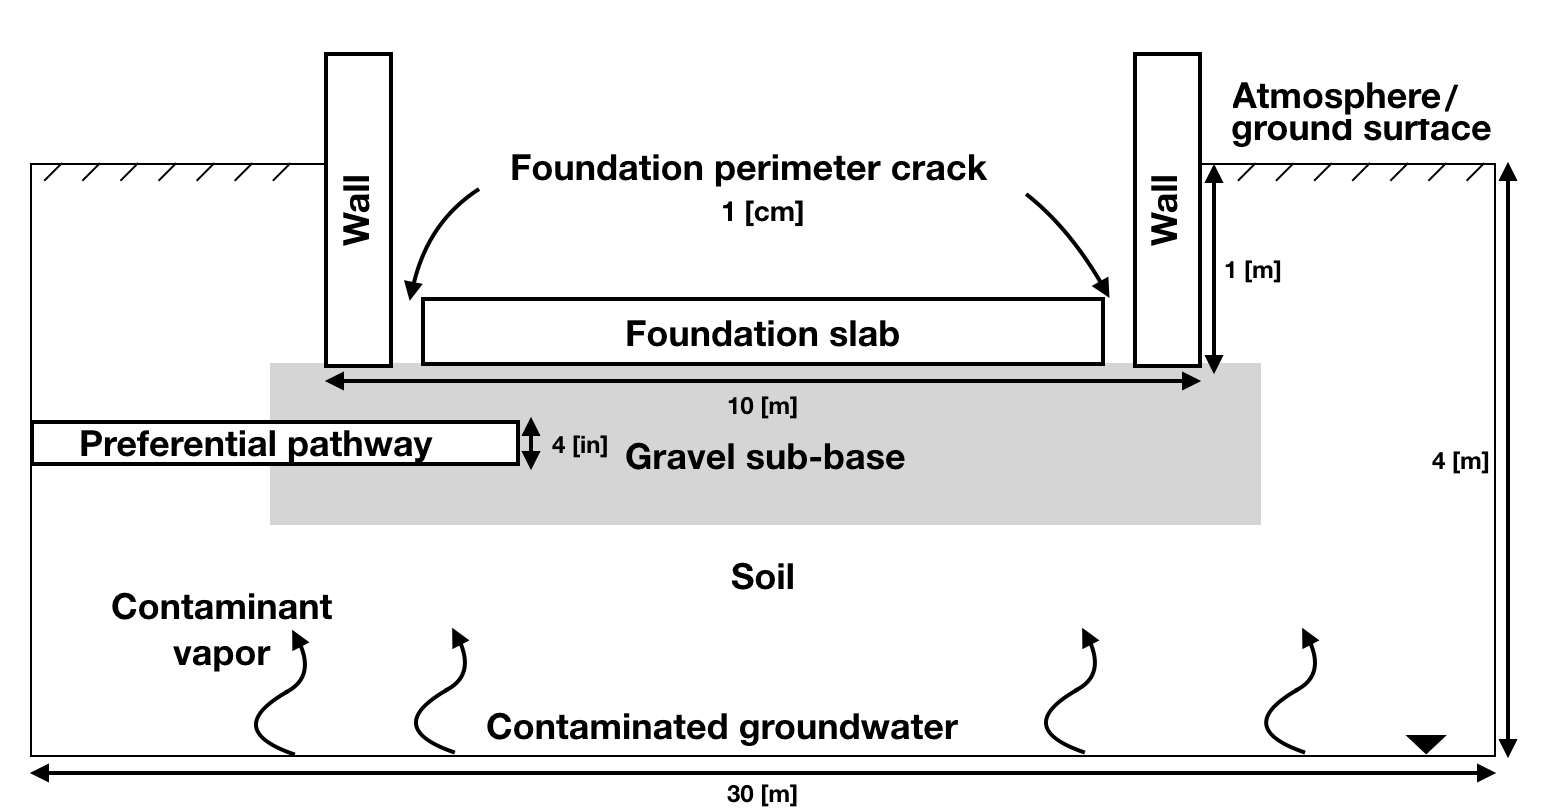
\includegraphics{model.png}
\end{figure}

In addition to examining the actual field data, a previously described three -dimensional computational fluid dynamics model of a generic VI impacted house was used to elucidate certain aspects of  the processes.
This model was implemented in a finite element solver package, COMSOL Multiphysics.
In the present work, there has been an addition of a preferential pathway to the ”standard” model that has been described before in publications by this group\cite{shen_influence_2013,yao_investigating_2017,yao_three-dimensional_2017}.
As in the earlier studies, only the vadose zone soil domain is directly modeled.

The modeled structure is assumed to have a 10x10 m foundation footprint, with the bottom of the foundation slab lying 1 m below ground surface (bgs), simulating a house with a basement.
The indoor air space is modeled as a continuously stirred tank (CST)\cite{u.s._environmental_protection_agency_oswer_2015} and all of the contaminant entering the house is assumed to enter with soil gas through a 1 cm wide crack located between the foundation walls and the foundation slab around the perimeter of the house.
All of the contaminant leaving the indoor air space is assumed to do so via air exchange with the ambient.
The indoor control volume is assumed to consist of only of the basement, assumed as having a total volume of $300 \; \mathrm{m^3}$.
Clearly different assumptions could be made regarding the structural features and the size of the crack entry route, but for present purposes, this is unimportant as the intent is only to show for “typical” values what the influence of certain other features can be. \par

The modeled surrounding soil domain extends 5 meters from the perimeter of the house, and is assumed to consist of sandy loam (except as noted).
Directly beneath the foundation slab, there is assumed to be a 30 cm (one foot) thick gravel layer, except in certain cases where this sub-base material is assumed to be the same as the surrounding soil (termed  a ”uniform” soil scenario). \par

Where relevant The preferential pathway is modeled as a 10 cm (4”) pipe that exits into the gravel sub-base beneath the structure.
The air in the pipe is assumed to be contaminated with TCE at a vapor concentration equal to the vapor in equilibrium with the groundwater contaminant concentration below the structure, modified by a scaling factor $\chi$, allowing the contaminant concentration in the pipe to be parameterized. \par

The groundwater beneath the structure is assumed to be homogeneously contaminated with trichloroethylene (TCE) as a prototypical contaminant.
The groundwater itself is not modeled, as the bottom of the model domain is defined by the top of the water table.
The ground surface and the pipe are both assumed to be sources of air to the soil domain.
Both are assumed to be at reference atmospheric pressure. \par

Vapor transport in the soil is governed by Richard’s equation, a modified version  of Darcy’s Law, taking the variability of soil moisture in the vadose zone into account\cite{richards_capillary_1931}.
The van Genuchten equations are used to predict the soil moisture content and thus the effective permeability of the soil\cite{van_genuchten_closed-form_1980}.
The effective diffusivity of contaminant in soil is calculated using the Millington-Quirk model\cite{millington_permeability_1961}.
The transport of vapor contaminant in the soil is assumed to be governed by the advection-diffusion equation, in which either advection or diffusion may dominate depending upon position and particular circumstances.
The equations and the boundary conditions are given in Table \ref{tbl:eqns-bc-parameters}.

\begin{table}[htb!]
  \centering
  \caption{Governing equations, boundary conditions \& model input parameters. (See below for table of nomenclature).}
  \label{tbl:eqns-bc-parameters}
  \bigskip
  %%%%%%%%%%%%%%%%%%%%%%%%%%%%%%%%%%%%%%%%%%%%%%%%%%%%%%%%%%%%%%%%%%%%%%%%%%%%%%
  % Governing equations
  %%%%%%%%%%%%%%%%%%%%%%%%%%%%%%%%%%%%%%%%%%%%%%%%%%%%%%%%%%%%%%%%%%%%%%%%%%%%%%
  \subcaption{Governing equations}
  \begin{tabular}{l l}
    \toprule
    % Indoor air space equation
    Unsteady-CSTR                 & $V\frac{d u}{d t} = \int_{A_\mathrm{ck}} j_\mathrm{ck} dA - u A_e V$ \\
    % Richard's equation
    Richard's equation            & $\nabla \cdot \rho \Big( - \frac{\kappa_s}{\mu} k_r \nabla p \Big) = 0$ \\
    % Millington-Quirk equation
    Millington-Quirk              & $D_\mathrm{eff} = D_\mathrm{air}\frac{\theta_g^{10/3}}{\theta_t^2} + \frac{D_\mathrm{water}}{K_H} \frac{\theta_w^{10/3}}{\theta_t^2}$ \\
    % Advection-diffusion equation
    Advection-diffusion equation  & $\frac{\partial}{\partial t} \Big( \theta_w c_w + \theta_g c \Big) = \nabla (D_\mathrm{eff} \cdot \nabla c) - \vec{u} \cdot \nabla c$ \\
    % van Genuchten's equations
    \multirow{3}{*}{van Genuchten equations}     & $\mathrm{Se} = \frac{\theta_w - \theta_r}{\theta_t - \theta_r} = [1 + |\alpha z|^n]^{-m}$ \\
                                  & $\theta_g = \theta_t - \theta_w$ \\
                                  & $k_r = (1 - \mathrm{Se})^{l} [1 - (\mathrm{Se}^{-m})^m]^2$ \\
                                  & $m = 1 - 1/n$ \\
    \bottomrule
  \end{tabular}
  \bigskip
  %%%%%%%%%%%%%%%%%%%%%%%%%%%%%%%%%%%%%%%%%%%%%%%%%%%%%%%%%%%%%%%%%%%%%%%%%%%%%%
  % Boundary conditions
  %%%%%%%%%%%%%%%%%%%%%%%%%%%%%%%%%%%%%%%%%%%%%%%%%%%%%%%%%%%%%%%%%%%%%%%%%%%%%%
  \subcaption{Boundary conditions}
  \begin{tabular}{l l l}
    \toprule
    \textbf{Boundary}          & \textbf{Richard's equation}      &   \textbf{Advection-diffusion equation} \\
    % Foundation crack
    At foundation crack  & $p = p_\mathrm{in/out} \; \mathrm{(Pa)}$                            & $j_\mathrm{ck} = \frac{u c}{1 - \exp{(u L_\mathrm{slab}/D_\mathrm{air})}}$ \\
    % Groundwater source
    At groundwater source &  N/A & $c = c_\mathrm{gw} K_H \; \mathrm{(\mu g/m^3)}$ \\
    % Ground surface
    At ground surface      & $p = 0 \; \mathrm{(Pa)}$  & $c = 0 \; \mathrm{(\mu g/m^3)}$ \\
    % Preferential pathway
    Exit of preferential pathway  & $p = 0 \; \mathrm{(Pa)}$  & $c = c_\mathrm{gw} K_H \chi \; \mathrm{(\mu g/m^3)}$ \\
    \bottomrule
  \end{tabular}
  \bigskip
  %%%%%%%%%%%%%%%%%%%%%%%%%%%%%%%%%%%%%%%%%%%%%%%%%%%%%%%%%%%%%%%%%%%%%%%%%%%%%%
  % Soil input parameters
  %%%%%%%%%%%%%%%%%%%%%%%%%%%%%%%%%%%%%%%%%%%%%%%%%%%%%%%%%%%%%%%%%%%%%%%%%%%%%%
  \subcaption{Soil \& gravel properties\cite{dan_capillary_2012,abreu_conceptual_2012,u.s._environmental_protection_agency_userss_2004}}
  \begin{tabular}{l l l l l l l}
    \toprule
    % Descriptions
    Soil & $\text{Permeability} \; \mathrm{(m^2)}$  & $\mathrm{Density} \; \mathrm{(kg/m^3)}$  & $\theta_s$  & $\theta_r$  & $\alpha \; \mathrm{(1/m)}$  & $n$ \\
    % Gravel
    Gravel     & $1.3 \cdot 10^{-9}$   & 1680    & 0.42        & 0.005       & 100       & 3.1 \\
    % sandy loam
    Sandy Loam    & $5.9 \cdot 10^{-13}$  & 1460    & 0.39        & 0.039        & 2.7       & 1.4 \\
    \bottomrule
  \end{tabular}
  \bigskip
  %%%%%%%%%%%%%%%%%%%%%%%%%%%%%%%%%%%%%%%%%%%%%%%%%%%%%%%%%%%%%%%%%%%%%%%%%%%%%%
  % TCE input parameters
  %%%%%%%%%%%%%%%%%%%%%%%%%%%%%%%%%%%%%%%%%%%%%%%%%%%%%%%%%%%%%%%%%%%%%%%%%%%%%%
  \subcaption{Trichloroethylene (diluted in air) properties\cite{abreu_conceptual_2012,u.s._environmental_protection_agency_userss_2004}}
  \begin{tabular}{l l l l l l}
    \toprule
    $D_\mathrm{air} \; \mathrm{(m^2/h)}$  & $D_\mathrm{water} \; \mathrm{(m^2/h)}$  & $\mathrm{Density} \; \mathrm{(kg/m^3)}$ & $\mathrm{Viscosity} \; \mathrm{(Pa \cdot s)}$  & $K_H$ & $M \; \mathrm{(g/mol)}$ \\
    $2.47 \cdot 10^{-2}$  & $3.67 \cdot 10^{-6}$  & 1.614 & $1.86 \cdot 10^{-5}$  & 0.403 & 131.39 \\
    \bottomrule
  \end{tabular}
  \bigskip
  %%%%%%%%%%%%%%%%%%%%%%%%%%%%%%%%%%%%%%%%%%%%%%%%%%%%%%%%%%%%%%%%%%%%%%%%%%%%%%
  % Building input parameters
  %%%%%%%%%%%%%%%%%%%%%%%%%%%%%%%%%%%%%%%%%%%%%%%%%%%%%%%%%%%%%%%%%%%%%%%%%%%%%%
  \subcaption{Building properties}
  \begin{tabular}{l l l}
    \toprule
    $V_\mathrm{base} \; \mathrm{(m^3)}$  & $L_\mathrm{slab} \; \mathrm{(cm)}$  & $A_e \; \mathrm{(1/hr)}$ \\
    %
    300  &  15  & 0.5 \\
    \bottomrule
  \end{tabular}
\end{table}

\section{Results \& Discussion}

\subsection{Statistical Analysis of Field Data}

\begin{figure}[htb!]
		\centering
    \caption{2D-KDE plot showing the distributions of indoor air contaminant concentration, the indoor/outdoor pressure difference, and how they correlate to each other.}
    \label{fig:kde}
    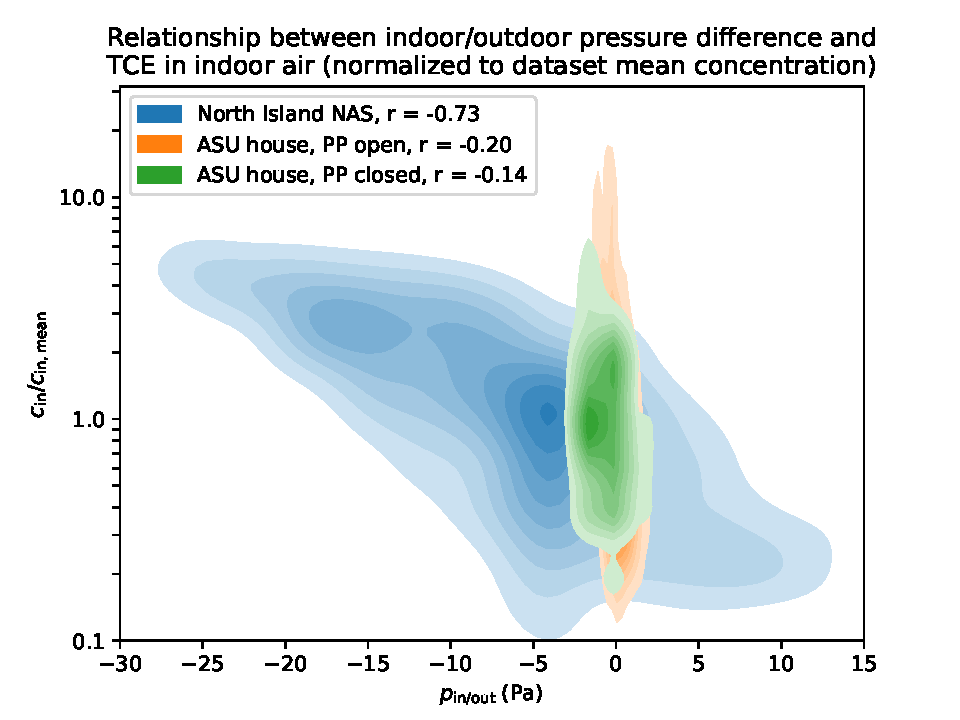
\includegraphics[width=\textwidth]{nas_asu_pp.pdf}
\end{figure}

\begin{table}[htb!]
  \caption{5th and 95th percentile values of $p_\mathrm{in/out}$ and $c_\mathrm{in}/c_\mathrm{in,mean}$ in Figure \ref{fig:kde}.}\label{tbl:percentiles}
  \begin{tabular}{c c c c c c c}
    \toprule
    & \multicolumn{2}{c|}{\textbf{North Island NAS}} & \multicolumn{2}{c|}{\textbf{ASU house PP Open}} & \multicolumn{2}{c}{\textbf{ASU House PP Closed}} \\
    Percentile & 5th & 95th & 5th & 95th & 5th & 95th \\
    $p_\mathrm{in/out}$ (Pa) & -19.9 & 7.4 & -1.4 & 2.1 & -2.1 & 2.27 \\
    $c_\mathrm{in}/c_\mathrm{in,mean}$ & 4.1 & 0.2 & 13.5 & 0.2 & 3.3 & 0.4 \\
    \bottomrule
  \end{tabular}
\end{table}

The pressure difference between the indoor and outdoor/ambient ($p_\mathrm{in/out}$) is an important driving force in VI, drawing in (or preventing) contaminants from entering a structure. % TODO: Add references
Changes in $p_\mathrm{in/out}$ is also a dynamic and fast process, impacting VI more rapidly than e.g. fluctuations in groundwater depth or contaminant concentration does; these processes may take weeks or even months to impact the overlying structure.
Therefore, it is reasonable to assume that the temporal variability in indoor air contaminant concentration $c_\mathrm{in}$ may be driven by changes in $p_\mathrm{in/out}$.

We examine the relationship between $p_\mathrm{in/out}$ and $c_\mathrm{in}$ by constructing the two-dimensional kernel density estimation (KDE) plots seen in Figure \ref{fig:kde}.
The KDE plots allow us to view the distribution of $p_\mathrm{in/out}$ and $c_\mathrm{in}$, and how well these correlate.
For this analysis we consider two VI sites, North Island NAS, and the ASU house, with the ASU house dataset divided up into two periods, before and after the land drain (called preferential pathway (PP) from here on) had been closed.
The preferential pathway significantly impacted the ASU house to such an extent that these two periods can essentially be considered as two different VI sites, and allowing us to examine the impact of the preferential pathway.

In Figure \ref{fig:kde}, the indoor air contaminant concentration $c_\mathrm{in}$ is normalized to the mean $c_\mathrm{in,mean}$ of each dataset, allowing us to compare the impact $p_\mathrm{in/out}$ had on $c_\mathrm{in}$.
A value of 10 on the y-axis indicate that $c_\mathrm{in}$ is 10 times greater than the mean here, and 0.1 indicate that it is one tenth of the mean.
The Pearson's r between $p_\mathrm{in/out}$ and $c_\mathrm{in}$ for each dataset is shown in the legend.

An interesting aspect of the North Island NAS site is that $p_\mathrm{in/out}$ varies so significantly, and the 5th and 95th percentile of $p_\mathrm{in/out}$ are -19.9 and 7.4 Pa respectively.
This may be contrasted with 5th and 95th percentile $p_\mathrm{in/out}$ at the ASU house: -1.4 and 2.1 Pa (PP open), and -2.1 and 2.27 Pa (PP closed).

The large (roughly one order of magnitude) under- and overpressurization of the North Island NAS site leads to roughly a one order magnitude increase and decrease from the mean $c_\mathrm{in}$.
Combined with $r=-0.73$, it is quite clear that at this site $p_\mathrm{in/out}$ largely determines $c_\mathrm{in}$ (there is still variability in $c_\mathrm{in}$ for a given $p_\mathrm{in/out}$, which we address later).
This is the same principle that governs the controlled pressure method (CPM) concept.

Turning to the ASU house datasets, we see a quite different situation.
The variability of $c_\mathrm{in}$ is just as large, or even larger than at North Island NAS, yet the $p_\mathrm{in/out}$ varies far less.
At first glance it may seem like the $c_\mathrm{in}$ values for the periods when the PP is open and closed respectively are relatively comparable, but the 5th and 95th percentiles values of differ significantly $c_\mathrm{in}/c_\mathrm{in,mean}$ as may be seen in Table \ref{tbl:percentiles}.

It is clear that the preferential pathway dramatically increases the ASU house's sensitivity to $p_\mathrm{in/out}$, and the site is fundamentally different during the period when the preferential pathway was open.
Yet, the magnitude of change in $c_\mathrm{in}$ is far greater than the change in $p_\mathrm{in/out}$, leading to the conclusion that it is not just increased flow rates into the structure that causes this, but there must also be an increased amount of contaminant as well as a much larger spatial variability in the sub-base.
This is a topic that we will return to later.

The magnitude of change in $c_\mathrm{in}$ when the PP is closed is more in line with the magnitude of change in $p_\mathrm{in/out}$, but there is still more variability than one would expect.
We hypothesize that this is largely due to fluctuations in air exchange rate, which we will examine later.

\subsection{Change In Indoor Air Contaminant Concentration Over Time} % TODO: Improve title

\begin{figure}[htb!]
  \centering
  \caption{Maximum change in indoor air contaminant concentration that may be expected over a given time period. (1D is 1 day, 2W is 2 weeks, and 3M is 3 months). The error bars are the 95\% confidence intervals.}
  \label{fig:resampling}
  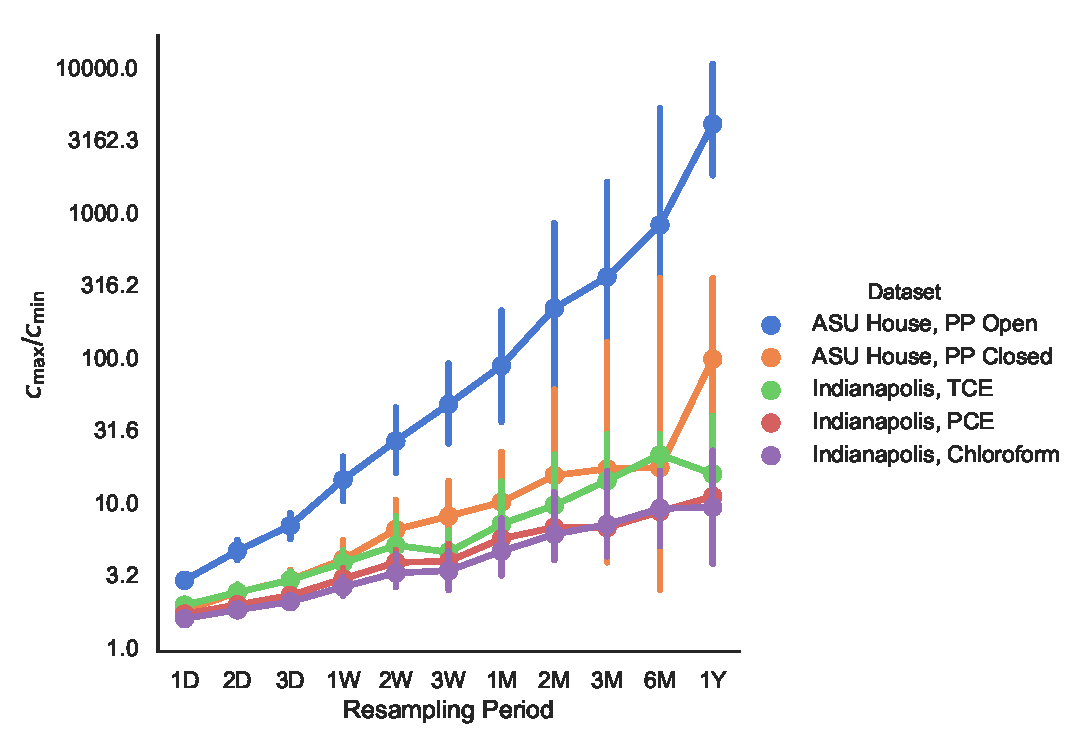
\includegraphics[width=\textwidth]{temporal_variability/resampling.pdf}
\end{figure}

% RESAMPLING TIME ANALYSIS
So far we have discussed how the relationship between $c_\mathrm{in}$ and $p_\mathrm{in/out}$, and how significantly $c_\mathrm{in}$ may vary at a site.
But this tells us little about how much variability in $c_\mathrm{in}$ may be expected over time.
For this analysis we turn to the ASU house data (PP open/closed considered separately again), and another well-studied VI site, the Indianapolis site in Indiana.
Both of these sites collected high frequency $c_\mathrm{in}$ samples over a significant periods and are therefore suitable for this analysis\cite{u.s._environmental_protection_agency_assessment_2015,holton_temporal_2013}.
Furthermore, at Indianapolis site the $c_\mathrm{in}$ of three different contaminants, Chloroform, Trichloroethylene (TCE), and Tetrachloroethylene (PCE) were collected, allowing us to see if there is any difference in the variability of each.
The North Island NAS dataset only spans a few days, and is therefore excluded from this analysis.

To demonstrate how significantly $c_\mathrm{in}$ can vary across time, we calculate the quotient of the maximum and minimum $c_\mathrm{in}$ (denoted as $c_\mathrm{max}/c_\mathrm{min}$) over a given time period.
I.e. if $c_\mathrm{in}$ samples were collected every four hours over a period of a year, and the data is resampled on a daily basis, then $c_\mathrm{max}/c_\mathrm{min}$ is returned for within each day, giving 365 data points.
Resampling periods of one, two, three, days, weeks, and months are chosen and Figure \ref{fig:resampling} shows the result of this analysis.

As one might expect, the longer the resampling period, the larger the maximum variability is: spanning from less than a threefold difference, to two to three orders of magnitude.
That such a large variability is observed when the resampling time approaches the length of the entire datasets is hardly surprising, nor is it surprising that the variability is much more significant when the preferential pathway was open than closed.
What may be surprising is that absent a preferential pathway such as the one at the ASU house, it may take a few weeks before an order of magnitude maximum variability is reached.
The most significant result of this analysis is that the maximum variability is quite small across a few days, suggesting that e.g. 24-hour passive samplers will resolve the daily temporal variability in $c_\mathrm{in}$ well ($c_\mathrm{max}/c_\mathrm{min} \approx 1.5$) and that a sampling frequency greater than a few days may yield little extra information.
There is also little difference between maximum variability of $c_\mathrm{in}$ the ASU house (when the PP is closed), and the three contaminants at the Indianapolis site, suggesting that this may be an "usual" amount of variability over these time periods.

\subsection{Variability Of Attenuation From Subslab}

\begin{figure}[htb!]
  \caption{Boxplot of attenuation from subslab at the ASU house site. The box shows the quartiles of the distribution, the whiskers the extent of the distribution, and diamonds are points that are considered outlier.}\label{fig:attenuation_subslab}
  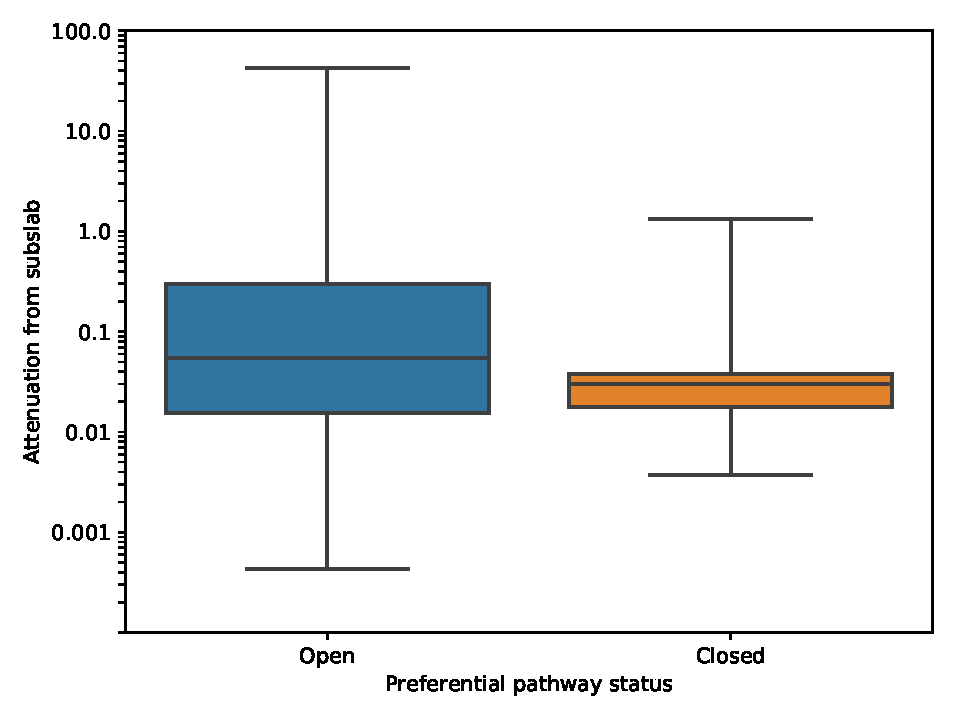
\includegraphics[width=0.7\textwidth]{asu_attenuation_subslab.pdf}
\end{figure}

To examine how $p_\mathrm{in/out}$ affects the contaminant entry rate (and subsequently the indoor air contaminant concentration) it would be convenient to analyze how $p_\mathrm{in/out}$ is correlated with the attenuation from subslab ($\alpha_\mathrm{subslab} = c_\mathrm{in}/c_\mathrm{subslab}$) at a site - in particularly for understanding how the PP at the ASU house affected the site dynamics.
By normalizing the $c_\mathrm{in}$ to $c_\mathrm{subslab}$ the $p_\mathrm{in/out}$ influence on the contaminant availability in the subslab area is mitigated.

The $c_\mathrm{subslab}$ are taken from the soilgas probe labeled as "6" at the ASU house, which is the probe located closest to the preferential pathway, and to a reported breach in the foundation\cite{guo_identification_2015}.
However, as Figure \ref{fig:attenuation_subslab} shows, there are some issues with using $\alpha_\mathrm{subslab}$ for subsequent analysis.

First, we can state that during the period when the preferential pathway was closed, $\alpha_\mathrm{subslab}$ does not vary that significantly, and is mostly around the EPA recommended $\alpha_\mathrm{subslab}$ value of 0.03\cite{u.s._environmental_protection_agency_oswer_2015}.
During the period when the preferential pathway was open, there is considerably more variability, and it is not uncommon for the $\alpha_\mathrm{subslab}$ to exceed unity.

Even though probe "6" is located in such close proximity to the preferential pathway, and the breach in the foundation, the contaminant concentration 'hotspot' is still missed.
This suggests that a preferential pathway may have an extremely localized influence in the subslab region, causing significant spatial variability in $c_\mathrm{subslab}$.
This shows how difficult it may be to locate a preferential pathway through subslab soilgas sampling.

The large $\alpha_\mathrm{subslab}$ values (compared to the recommended EPA value of 0.03) can often indicate that there may be indoor sources present a site, which there were none of at the ASU house.
Thus, in addition to potentially indicating indoor contaminant sources, large $\alpha_\mathrm{subslab}$ may also indicate the presence of a preferential pathway.

\subsubsection{Modeling Results} % TODO: Improve title

\begin{figure}[htb!]
	\centering
  \caption{Simulated preferential pathway scenarios compared to ASU house field data (top panel). No preferential pathway scenarios in bottom panel. Field data is binned in 40 evenly spaced bins, with the dot representing the mean and errors bars one standard deviation for that binned mean.}
  \label{fig:land_drain_scenarios}
  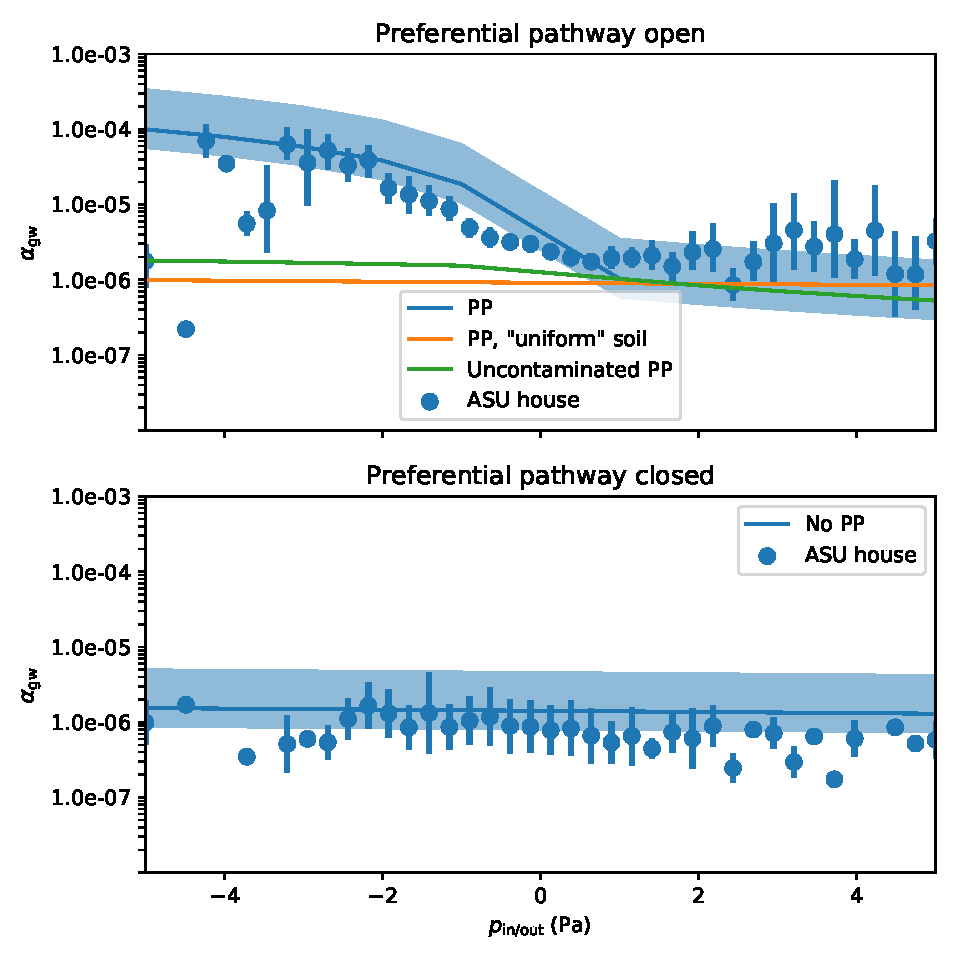
\includegraphics[width=\textwidth]{land_drain_scenarios_combo.pdf}
\end{figure}

To begin a more thorough discussion regarding the role and impact a preferential pathway may have at a particular site, we turn to our model presented in the methods section.
Here, $A_e$ is assumed to be a constant 0.5 per hour, and $p_\mathrm{in/out}$ is varied from -5 to 5 Pa.
The predicted $c_\mathrm{in}$ is then normalized to the groundwater concentration $c_\mathrm{gw}$, giving the attenuation from groundwater $\alpha_\mathrm{gw}$.

The predicted $\alpha_\mathrm{gw}$ as a function of $p_\mathrm{in/out}$ is given by the central blue line in the upper panel of Figure \ref{fig:land_drain_scenarios} (ignore the shaded blue areas for now).
These predicted values are compared to $\alpha_\mathrm{gw}$ from the ASU house data from the period the preferential pathway was open, given by the blue dots.

The model successfully predicts the increase in $\alpha_\mathrm{gw}$ as $p_\mathrm{in/out}$ decreases (increased depressurization) but somewhat underpredicts $\alpha_\mathrm{gw}$ as the house is overpressurized.
Most significantly, the model captures that even for a small increase in depressurization (0 to -5 Pa) a very large increase in $\alpha_\mathrm{gw}$ (two order of magnitude) occurs.
This asymmetry is due to two factors.

First, the preferential pathway acts as preferential air source, circumventing the large resistance to flow in the surrounding soil, and allowing a small change in $p_\mathrm{in/out}$ to much more dramatically increase the advective flow into the structure from the subslab region.
A second simulation, where the model is rerun with the preferential pathway present, but the permeable (gravel) layer in the subslab is removed and instead is assumed to be of the same material as the surrounding soil (sandy loam), giving a "uniform soil" scenario (orange line in the top panel of Figure \ref{fig:land_drain_scenarios}).
This simulation demonstrates that without a permeable subslab to effectively allow the "advective potential" to be realized, a preferential pathway may not impact a VI site; a preferential pathway requires good communication between the indoor environment and itself to be as a significant contributor to VI as was seen at the ASU house site.

The second factor is that the preferential pathway must contain contaminant vapors to be impactful.
In a third simulation, the permeable subslab region is included, but the preferential pathway is filled with clean air, i.e. just allows the "advective potential" to be realized, but without any additional contaminant introduced.
The result of this simulation is given by the green line in the top panel of Figure \ref{fig:land_drain_scenarios}.
This shows that while there was a slightly larger increase in $\alpha_\mathrm{gw}$ compared to the "uniform soil" scenario as the structure is increasingly depressurized, it is nowhere near as significant as when the preferential pathway was filled with contaminant vapors.
The contaminated and uncontaminated preferential pathway scenarios (blue and green lines respectively) thus give the range of $\alpha_\mathrm{gw}$ that one may see for a given $p_\mathrm{in/out}$ depending on the contaminant vapor concentration in the preferential pathway.

The model is also able to capture $\alpha_\mathrm{gw}$ as a function of $p_\mathrm{in/out}$ when a preferential pathway is absent (but there is a permeable subslab region), as the bottom panel in Figure \ref{fig:land_drain_scenarios} shows.
However, what these simulations fail to predict is the considerable variability of $\alpha_\mathrm{gw}$ for a given $p_\mathrm{in/out}$, as shown by the error bars in the two panels (denoting one standard deviation).
A significant portion of this variability may be explained by variation in air exchange rate, $A_e$.

Air exchange rate determines which portion of the indoor is exchanged with outdoor air, reducing the indoor air contaminant concentration.
A high air exchange is associated with lower $c_\mathrm{in}$ and low with higher $c_\mathrm{in}$.
$A_e$ is correlated with $p_\mathrm{in/out}$, i.e. that a depressurized structure has higher $A_e$ than an overpressurized structure as more air from the outside may be brought in, but with significant variability.
Determining any determinant relationship between $A_e$ and $p_\mathrm{in/out}$ is difficult: the structure itself and weather phenomena has a huge effect on air exchange, i.e. for a given $p_\mathrm{in/out}$.
Fortunately, the range of $A_e$ values are typically bounded, with the U.S. EPA reporting that (depending on region) the 10th percentile values range from 0.16 to 0.2 per hour, and the 50th and 90th percentiles range from 0.35 to 0.49 and 1.21 to 1.49 per hour respectively\cite{u.s._epa_exposure_2011,m._d._koontz_estimation_1995}.
These values are in line with what as found at the both the ASU house and the Indianapolis site as Table \ref{tbl:air_exchange_rate} shows.

To more accurately predict the range of $\alpha_\mathrm{gw}$ values for a given $p_\mathrm{in/out}$, the preferential pathway (top panel, blue line) and the no preferential pathway (bottom panel, blue line) scenarios are rerun with $A_e$ equal to 0.1, 0.5, and 1.5 per hour, giving us a predicted upper and lower bound for $\alpha_\mathrm{gw}$.
These bounds are given by the blue region above and below the central line, with the upper and lower bound associated with 0.1 and 1.5 air exchange rate per hour respectively.
Doing this allows us to capture most of the variability in $\alpha_\mathrm{gw}$, indicating that a significant portion of the variability in $\alpha_\mathrm{gw}$ for a given $p_\mathrm{in/out}$ may be attributed to fluctuations in air exchange rate.
This could be used during VI site investigations to estimate how significantly the indoor air contaminant concentration may fluctuate.

\begin{table}[htb!]
  \caption{Air exchange rate values (1/hr)}\label{tbl:air_exchange_rate}
  \begin{tabular}{l c c c}
    \toprule
    \textbf{Percentile} & \textbf{10th} & \textbf{50th} & \textbf{90th} \\
    EPA\cite{u.s._epa_exposure_2011,m._d._koontz_estimation_1995} & 0.16-0.2 & 0.35-0.49 & 1.21-1.49 \\
    ASU house\cite{holton_temporal_2013,guo_identification_2015} & 0.21 & 0.43 & 0.78 \\
    Indianapolis\cite{u.s._environmental_protection_agency_assessment_2015} & 0.34 & 0.74 & 1.27 \\
    \bottomrule
  \end{tabular}
\end{table}

\begin{acknowledgement}
  This project was supported by grant ES-201502 from the Strategic Environmental Research and Development Program and Environmental Security Technology Certification Program (SERDP-ESTCP).
\end{acknowledgement}

\bibliography{library}

\end{document}
